\documentclass[a4paper,12pt]{article}
\usepackage[spanish]{babel}
\usepackage[utf8]{inputenc}
\usepackage[pdftex]{graphicx}
\usepackage{float}
\graphicspath{ {img/} }
\begin{document}
\title{ESTRATEGIA DE SEGURIDAD PARA INTERNET Y EXTRANE EN EMPRESAS}
\author{Jorge Chicala Arroyave}
\date{\today}
\maketitle
\begin{bf}
URL del Repositorio:
\end{bf}
https://github.com/jchicala/proyecto\_final
\begin{bf}
\begin{center}
RESUMEN \\
\end{center}
\end{bf}
Con el crecimiento de la tecnología de información y la ubicuidad de los medios
de difusión y comunicación empresariales (Intranet y Extranet), es cada vez más
necesaria adecuadas medidas de seguridad de la información y en especial la 
implementación de un Sistema de Gestión de la Seguridad de la Información (SGSI).
 Una metodología adecuada en la cual se identifiquen los riesgos, se generen el 
diseño de seguridades y se asegure la memoria técnica de los procesos y el 
accionar de seguridad en el día a día, se hace necesaria, como un mecanismo para asegurar el cumplimiento de la seguridad de información.\\   
\break
\begin{bf}
Palabras claves:
\end{bf}
Intranet, Extranet, Seguridad, Octave, Magerit. \\
\begin{bf}
\begin{center}
INTRODUCCION\\
\end{center}
\end{bf}
Nos estamos ahogando en información, pero hambrientos de conocimientos. 
John Naisbitt, Megatrends.\\
Las organizaciones y los individuos, actualmente, enfrentan una avalancha de 
datos e información, las cuales, muchas veces pueden resultar críticas en su 
naturaleza de agente diferenciador de competitividad, pero a la vez, es difícil 
de administrar y asegurar apropiadamente.\\
Actualmente las empresas están enfocando sus esfuerzos en administrar, de la 
mejor manera posible, sus activos más valiosos, los primarios que abarca la 
información y los secundarios que son aquellas herramientas de soporte para la 
información, entre los que se incluyen el software, hardware, comunicación, 
usuarios y la estructura que los soporta.\\
Cualquier sistema informático que maneje información y que permita la comunicación 
para compartir esta información, es vulnerable a ataques informáticos, es por 
este motivo que, el análisis de riesgo, basado en una metodología que permita la identificación y valoración del riesgo se convierte en una herramienta 
de ayuda para la definición e implementación de políticas y procedimientos de 
seguridad.\\
\begin{bf}
\begin{center}
ESTADO DEL ARTE\\
\end{center}
\end{bf}
\begin{bf}   
Gestión del Riesgo\\
\end{bf}
\break
La definición ampliamente usada y promulgada por la Organización Internacional de 
Normalización (ISO), define la Gestión de Riesgo como “La posibilidad de que una 
amenaza determinada explote las vulnerabilidades de un activo o grupo de activos y 
por lo tanto causa daño a la organización” \cite{Institute2009}.
\begin{figure}[h!]
\centering
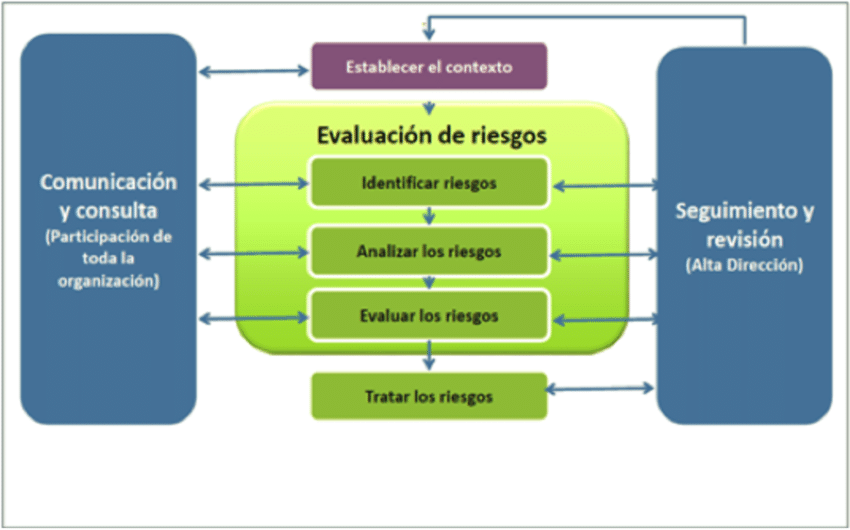
\includegraphics[width=5cm]{Manejo_Riesgo_ISO-31000.png}
\caption{Gestion del Riesgo - Flujo ISO 37001}
\end{figure}
La Gestión del Riesgo, conforme el estándar ISO 31000:2018 consta de los procesos indicados en la 
Fig1. \cite{Grupo2018}.
\begin{itemize} 
\item Comunicación y Consulta, asiste a las partes interesadas pertinentes a comprender el 
riesgo. 
\item Establecimiento del Contexto, adapta el proceso de gestión para un evaluación 
eficaz y procesamiento apropiado. 
\item Evaluación del Riesgo, comprende:
\begin{itemize}
\item Identificación del riesgo, cuyo objetivo es encontrar, reconocer y describir los 
riesgos que pueden ayudar o impedir a una organización lograr sus objetivos. 
\item Análisis del riesgo, su propósito es comprender la naturaleza del riesgo y sus 
características incluyendo, el nivel del riesgo. 
\item Valoración del riesgo, apoya a la toma de decisiones.
\end{itemize} 
\item Tratamiento del Riesgo, selecciona e implementa mecanismo para mitigar el riesgo. 
\item Seguimiento y Revisión, revisa cumplimiento, asegura y mejora la calidad de los 
procesos implementados. 
\item Registro e Informe, generación de memoria documental de los resultados de los 
procesos implementados.
\end{itemize}
\break
\begin{bf}
Intranet\\ 
\end{bf}
\break
Es una red de ordenadores con acceso restringido que solo pueden utilizar los 
usuarios autorizados de una empresa/institución/grupo y que fomenta el intercambio
de información entre los miembros de una empresa, con el objetivo fundamental de 
asegurar una comunicación fluida entre los empleados o entre empleados y clientes, 
de tal manera que puedan compartir de forma segura y rápida conocimientos e 
información dentro del grupo autorizado \cite{Cabello2014}.
Entre las características de una Intranet se encuentran: Confidencialidad, 
Integridad, Autenticación, Verificación, Disponibilidad.\\
\break 
\begin{bf}
Tipos de Intranet\\
\end{bf}
\begin{enumerate} 
\item Plataformas de colaboración, los empleados pueden realizar pregunta, buscar 
aclaraciones y tener conversaciones. Se pueden compartir documentos o herramientas 
institucionales.\\
\item Sitios Web Internos, accesibles solo para los usuarios de la empresa, consumidores
del contenido. Un grupo de administradores pueden crear, publicar, editar, 
eliminar contenidos.\\ 
\item Intranet Distribuida, para empresas grandes, permite descentralizar los servicios 
a la vez crear múltiples aplicaciones, recursos y herramientas con una 
infraestructura y diseño común de tal manera que le brinde autonomía dentro de la 
red privada de la empresa.\\
\end{enumerate}
\break 
\begin{bf}
Extranet\\
\end{bf}
\break
Es una red privada de ordenadores con acceso restringido que solo pueden utilizar 
los usuarios autorizados de una empresa/organización/institución/grupo y que 
fomenta el intercambio de manera segura de sus conocimientos, información y 
operaciones con un grupo selecto de interesados externos, quienes participan 
activamente de los procesos del negocio \cite{Cabello2014}. 
Entre las características de una Extranet se encuentran: Procesos y flujos de 
trabajo más ágiles, Proyectos y Aprendizajes en colaboración, Archivos y Documentos 
compartidos, Red de Computadoras.\\ 
\break
\begin{bf}  
Tipos de Extranet\\
\end{bf}
\break
\begin{enumerate}    
\item Extranet de Empresa a Consumidor, similar a un portal de clientes, en el cual se 
puede ingresar y comprobar el estado de pedidos. 
\item Extranet de Empresas/Socios Comerciales, definición de un espacio de colaboración 
de las partes interesadas. Información es compartida y visualizada en base a 
permisos.
\item Extranet de la Industria, creada por la empresa, para proveer accesos a herramientas 
y recursos, a la vez que facilita el intercambio de ideas en la industria con el objetivo de crear o proporcionar mejores productos o servicios.\\ 
\end{enumerate}
\bibliographystyle{apacite}
\bibliography{M6_Chicala_Arroyave_Jorge}
\end{document}
